\documentclass[final]{beamer}
\usepackage[orientation=portrait,size=a0,scale=1.425,debug]{beamerposter} % Format beamer as poster

\usepackage[ngerman,english]{babel}  % Language specification
\usepackage{varioref}  % Better references but possibly unstable
\usepackage[T1]{fontenc}  % Output umlauts in a PDF
\usepackage[utf8]{inputenc}
\usepackage{pslatex}
\usepackage{amsmath}
\usepackage{multirow}

\usepackage[font=small,labelfont=bf]{caption}  % Customize caption aesthetics
\usepackage[subrefformat=parens,labelformat=parens,font=small]{subcaption}  % Customize sub-captions

\usepackage{color}
\usepackage{xcolor}  % Highlighting
\usepackage{tcolorbox}  % Fancy colored boxes
\usepackage{soul}

\usepackage[tracking=true]{microtype}  % Change character spacing

\usepackage{graphicx}  % Insert images
\usepackage{listings}  % Insert programming code
\usepackage[space]{grffile}  % Insert images baring a filename which contains spaces
\usepackage{float}  % Forcefully set the location of an object

\usepackage[backend=biber,style=numeric,sorting=none,giveninits=true,doi=false,isbn=false,url=false,eprint=false]{biblatex}  % Reference manager
\usepackage{csquotes}		% Ensure proper quotation of texts with babel and polyglossia with biblatex
\usepackage{hyperref}		% Insert clickable references

\usepackage[nodayofweek]{datetime}  % Flexible date specification
\usepackage{scrextend}  % Arbitrary indentation

\AtBeginBibliography{\footnotesize}
\addbibresource{../literature.bib}

\captionsetup{font=small,skip=0em}  % Move caption close to figure and or graphic

\newcommand{\mathcolorbox}[2]{\colorbox{#1}{$\displaystyle #2$}}
\newcommand{\parvspace}[1]{\vspace{.5em}}  % Manually HACK space after a paragraph

\setbeamertemplate{navigation symbols}{}

% Prettify poster
\definecolor{TrinityBlue}{RGB}{32, 113, 182}
\usefonttheme[onlymath]{serif}%
\setbeamerfont{title}{size=\LARGE}
\setbeamercolor*{title}{fg = white}%
\setbeamercolor*{author}{fg = white}%
\setbeamercolor*{institute}{fg = white}%
\setbeamercolor*{date}{fg = white}%
\setbeamercolor*{title page}{fg = black}%
\setbeamercolor*{item}{fg = black}%
\setbeamercolor*{block title}{fg = TrinityBlue}%
\setbeamercolor*{caption name}{fg = black}%
\setbeamercolor*{bibliography item}{fg = black}
\setbeamercolor*{bibliography entry author}{fg = black}%
\setbeamercolor*{bibliography entry title}{fg = black}%
\setbeamercolor*{bibliography entry location}{fg = black}%
\setbeamercolor*{bibliography entry note}{fg = black}%
\setbeamerfont{title}{series = \bfseries}%
\setbeamerfont{institute}{size = \small}%
\setbeamertemplate{bibliography item}[text]
\setbeamertemplate{caption}[numbered]%
\setbeamertemplate{caption label separator}[endash]%
%\usebackgroundtemplate{\includegraphics[width=\paperwidth,height=\paperheight]{./MUW_green.pdf}}  % Background image

\title{Augmenting the DonorsChoose.org Corpus for Meta-Learning}
\subject{Algorithm Selection and Meta-Learning in Information Retrieval}
\author{Gordian~Edenhofer\inst{1,2} \and Andrew~Collins\inst{1} \and Akiko~Aizawa\inst{2} \and Joeran~Beel\inst{1,2}}
\institute{%
	\inst{1}Trinity College Dublin, School of Computer Science \& Statistics, ADAPT Centre, Ireland\\
	\inst{2}National Institute of Informatics Tokyo, Digital Content and Media Sciences Division, Japan
	\and \href{mailto:beelj@tcd.ie}{beelj@tcd.ie}, \href{mailto:ancollin@tcd.ie}{ancollin@tcd.ie}, \href{mailto:aizawa@nii.ac.jp}{aizawa@nii.ac.jp}
}
\date{\itshape{} Algorithm Selection and Meta-Learning in Information Retrieval (AMIR)}  % Set date to venue

\begin{document}

\begin{frame}[t,fragile=singleslide]{}
	% Headline
	\colorbox{TrinityBlue}{
		\hspace{-1.02em}  % Ugly HACK to center background block around header and avoid "overfull \hbox" message
		\begin{columns}[t]
			\begin{column}{0.01\textwidth}
			\end{column}

			\begin{column}{0.18\textwidth}
				\flushleft%
				\vspace{1em}
				
\includegraphics[width=0.75\columnwidth]{{{../res/Logo of Trinity College Dublin}}}
			\end{column}

			\begin{column}{0.5\textwidth}
				\vspace{1em}
				\titlepage{}
			\end{column}

			\begin{column}{0.18\textwidth}
				\flushright%
				\vspace{1em}
				\vspace{2em}
\includegraphics[width=0.8\columnwidth]{{{../res/Logo of ADAPT}}}
			\end{column}

			\begin{column}{0.01\textwidth}
			\end{column}
		\end{columns}
	}
	\vspace{0.em}  % HACK to leave some space between the header and the content

	\begin{columns}[t]
		\begin{column}{0.45\textwidth}
			\begin{block}{}
			The augmented dataset and the source code are released into the public domain at \colorbox{yellow}{\bfseries \href{https://github.com/BeelGroup/Augmented-DonorsChoose.org-Dataset}{GitHub:BeelGroup/Augmented-DonorsChoose.org-Dataset}}. Each feature worthy of an explanation is described in the repository.
			\end{block}
			\vspace{1.5em}

			\begin{block}{Introduction}
				Meta-Learning is the process of applying machine learning on metadata of previous machine learning experiments. The goal is to improve existing approaches by combining the strengths of several single machine learners. The metadata though needs to be computed in advance.
				\parvspace{}

				Multiple examples of manual and repetitious data augmentation may be found in the scientific literature, for instance in~\cite{CUNHA2018128,DBLP:journals/corr/abs-1805-12118,Ekstrand:2012:RFP:2365952.2366002}. Furthermore, the choice of the metric for computing metadata of single machine learners is important. Using the RMSE, as is done in some of the aforementioned publications, disallows using content-based methods.
				\parvspace{}

				Our objective is to address the data augmentation part in a comprehensive and reproducible~\cite{UMUAI:TowardsReproducibilityInRecSysBeel2016} way. We are augmenting a public domain dataset intrinsically about recommendations which to our best knowledge has not been used for meta-learning before in the scientific community. Yet due to its feature-rich and vast corpus is suitable.
			\end{block}
		\end{column}

		{
			\color{gray}
			\hspace{-1em}
			\vrule{}
			\hspace{+1em}
		}

		\begin{column}{0.45\textwidth}
			\begin{block}{Methodology}
				The DonorsChoose.org dataset is composed of past donations featuring $4.69$ million transactions performed by $2.12$ million users having donated to $1.11$ million projects. It provides more feature-richt transactions in contrast to, e.g., the popular MovieLens dataset as outlined in~\autoref{tab:IllustrativeTable}.
				\parvspace{}

				The augmented data which is to the right of the separator in~\autoref{tab:IllustrativeTable} is composed of the metadata of SVD, KNN, TF-IDF and word-embedding using fastText~\cite{scikit-learn,rehurek_lrec,DBLP:journals/corr/BojanowskiGJM16}. Vector representations of items are the normalized sum of the vectors of the normalized embeddings of the individual words. In order to work with the data in an efficient way, $100,000$ transactions are sampled.
				\parvspace{}

				The recall in a Top-N test set is used as score of how good an algorithm is able to recommend an item.
				\begin{enumerate}
					\item For each user, first $100$ items with which the user has not interacted are selected.
					\item The algorithm then ranks an item with which the user has interacted and the $100$ randomly sampled items.
					\item The position of the item with which the user has interacted in the ranked test set may now be taken as the recall in a Top-N test set.
				\end{enumerate}
			\end{block}
		\end{column}
	\end{columns}

	\begin{columns}[t]
		\begin{column}{0.645\textwidth}
			\begin{table}[ht]
				\centering
				\includegraphics[width=\textwidth,height=0.5\textheight,keepaspectratio]{{{../res/table}}}
				\caption{Illustrative example of the overall design of the augmented transaction table with amended learning subsystem performance scores, statistics and meta-learner information.}%
				\label{tab:IllustrativeTable}
			\end{table}
		\end{column}
	\end{columns}

	\begin{columns}[t]
		\begin{column}{0.945\textwidth}
			\color{gray}
			\vspace{0.5em}
			\hrule{}
			\vspace{0.5em}
		\end{column}
	\end{columns}

	\begin{columns}[t]
		\begin{column}{0.945\textwidth}
			\begin{block}{Results}
				\begin{columns}[t]
					\begin{column}{0.49\textwidth}
						The preparation of the dataset preserves a little more than half of the data with the most notable drop in the number of transactions being introduced by requiring users to have donated at least twice. The sample of $100,000$ transactions contains $18,735$ unique users and $88,100$ unique projects. The decay of the interaction frequency is seen in~\autoref{fig:InteractionFrequency}, the distribution of interaction strength in~~\autoref{fig:InteractionStrength}.

						\begin{figure}[ht]
							\centering
							\subcaptionbox{Interaction Frequency\label{fig:InteractionFrequency}}{
								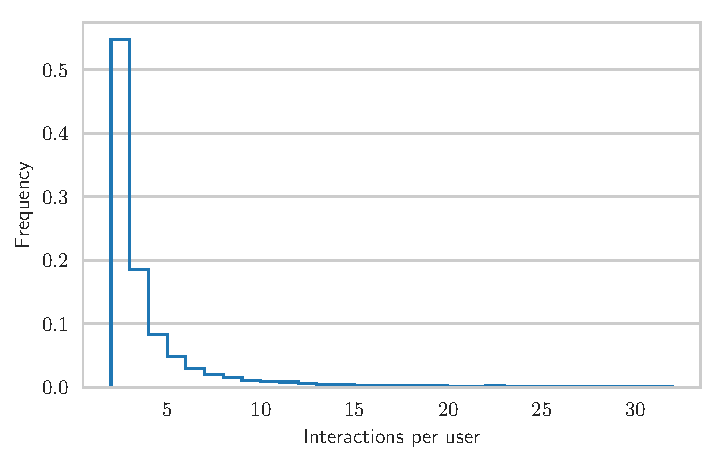
\includegraphics[width=0.45\textwidth,height=\textheight,keepaspectratio]{{{../res/number_interactions}}}
							}
							\hspace{.5em}
							\subcaptionbox{Interaction Strength\label{fig:InteractionStrength}}{
								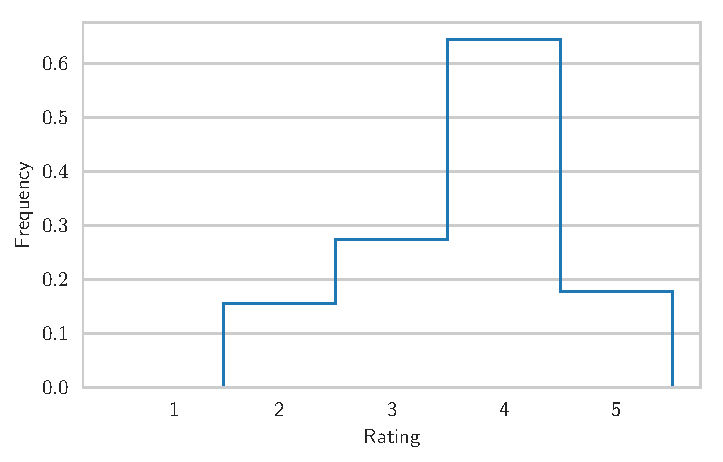
\includegraphics[width=0.45\textwidth,height=\textheight,keepaspectratio]{{{../res/distribtion_ratings}}}
							}
							\caption{The frequency of the number of interactions per user without outliers is shown in~\subref{fig:InteractionFrequency} and the distribution of the transformed interaction strength is shown in~\subref{fig:InteractionStrength}.}%
							\label{fig:Interactions}
						\end{figure}
					\end{column}

					\begin{column}{0.49\textwidth}
						Statistical features about the performances of the individual machine learners in the learning subsystem are visualized in~\autoref{fig:MetaLearnerStatistics}. Overall, content-based filters are significantly better in achieving a low recall-position. The baseline is set to be the single best algorithm, i.e., TF-IDF. As seen in~\autoref{fig:MetaLearnerPerformance}, the baseline is beaten by two meta-learners.

						\begin{figure}[ht]
							\centering
							\subcaptionbox{Statistics\label{fig:MetaLearnerStatistics}}{
								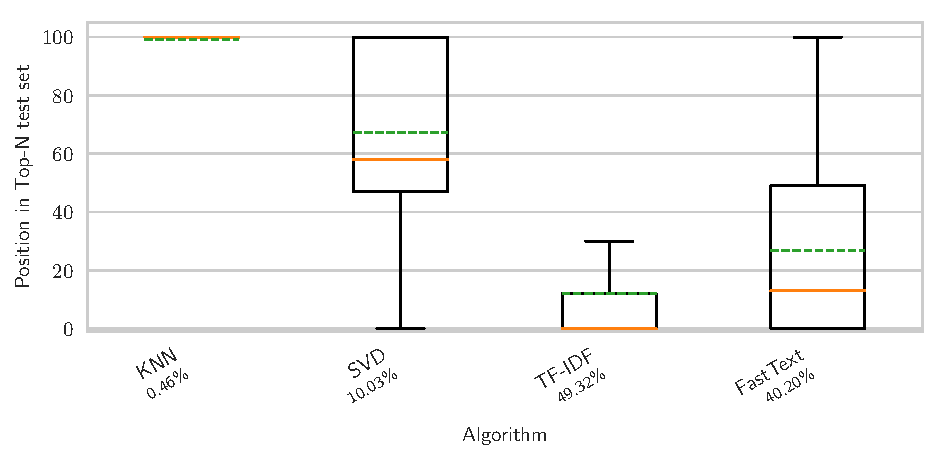
\includegraphics[width=.45\textwidth,height=\textheight,keepaspectratio]{{{../res/learning_subsystem_position}}}
							}
							\hspace{.5em}
							\subcaptionbox{Perfromance\label{fig:MetaLearnerPerformance}}{
								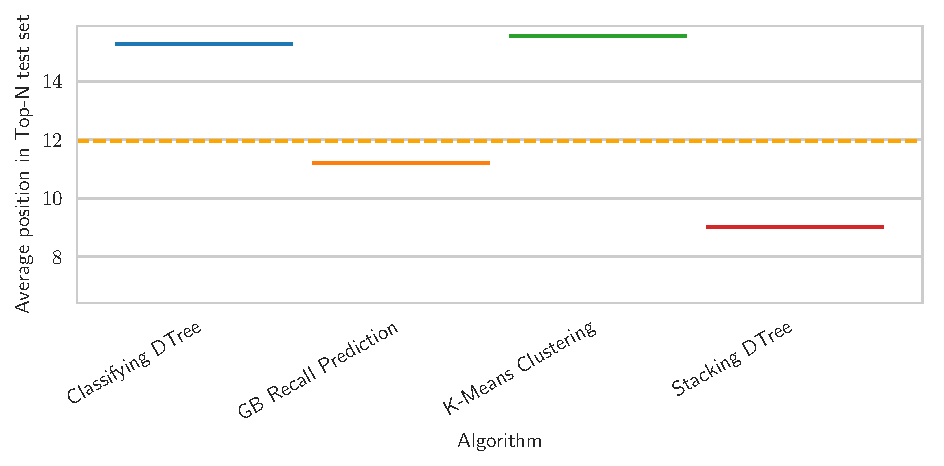
\includegraphics[width=.45\textwidth,height=\textheight,keepaspectratio]{{{../res/meta_learner_performance_average_position}}}
							}
							\caption{Statistical features of the recall-positions of the learning subsystem are shown in~\subref{fig:MetaLearnerStatistics}. The dashed green lines indicate the means, the straight orange lines the medians. The percentage below each algorithm indicates how often it is the best possible algorithm. To resolve a draw deterministically, the ``best'' algorithm is decided in alphabetic order.
							The performance of the meta-learner system is shown in~\subref{fig:MetaLearnerPerformance}. The dashed orange line represents the overall best algorithm, i.e., TF-IDF.}%
							\label{fig:MetaLearner}
						\end{figure}
					\end{column}
				\end{columns}
			\end{block}
		\end{column}
	\end{columns}

	\begin{columns}[t]
		\begin{column}{0.945\textwidth}
			\color{gray}
			\vspace{0.5em}
			\hrule{}
			\vspace{0.5em}
		\end{column}
	\end{columns}

	\begin{columns}[t]
		\begin{column}{0.45\textwidth}
			\begin{block}{Conclusion}
				The study provides an extensively augmented dataset based on the transaction data published by DonorsChoose.org. The corpus is amended with metadata of individual recommender algorithms. Collaborative and content-based filtering techniques are used in the process and their performance is evaluated via the recall in a Top-N test set. Aggregated user and item statistics are amended to the table. Furthermore, Metadata of four switching hybrid ensemble meta-learners is amended to the dataset. The augmented public domain dataset lays the groundwork that future evaluations of existing and novel meta-learning approaches can build upon.
			\end{block}

			\begin{block}{Acknoledgement}
				\footnotesize
				This publication emanated from research conducted with the financial support of Science Foundation Ireland (SFI) under Grant Number 13/RC/2106.
			\end{block}
		\end{column}

		{
			\color{gray}
			\hspace{-1em}
			\vrule{}
			\hspace{+1em}
		}

		\begin{column}{0.45\textwidth}
			\begin{block}{References}
				\printbibliography[heading=none]
			\end{block}
		\end{column}
	\end{columns}
\end{frame}

\end{document}
